
\subsection{Axis Descriptions}
Axis descriptions are labels for $x$ and $y$ axis, titles, legends and the like. Axis descriptions are drawn after the plot is finished and they are not subjected to clipping. 

\subsubsection{Placement of Axis Descriptions}
This section describes how to \emph{modify} the placement of titles, labels, legends and other axis descriptions. It may be skipped at first reading.

There are different methods to place axis descriptions. One of them is to provide coordinates relative to the axis' rectangle such that |(0,0)| is the lower left corner and |(1,1)| is the upper right corner -- this is very useful for figure titles or legends. Coordinates of this type, i.e.\ without unit like |(0,0)| or |(1.03,1)|, are called |axis description cs| (the |cs| stands for ``coordinate system''). One other method is of primary interest for axis labels -- they should be placed near the tick labels, but it a way that they don't overlap or obscure tick labels. Furthermore, axis labels shall be placed such that they are automatically moved if the axis is rotated (or tick labels are moved to the right side of the figure). There is a special coordinate system to realize these two demands, the |ticklabel cs|.

In the following, the two coordinate systems |axis description cs| and |ticklabel cs| are described in more details. It should be noted that |axis description cs| is used automatically, so it might never be necessary to use it explicitly.


\begin{coordinatesystem}{axis description cs}
\label{pgfplots:sec:axis:description:cs}
	A coordinate system which is used to place axis descriptions. Whenever the option `|at={(|\meta{x}|,|\meta{y}|)}|' occurs in |label style|, |legend style| or any other axis description, |(|\meta{x}|,|\meta{y}|)| is interpreted to be a coordinate in |axis description cs|.

	The point $(0,0)$ is always the lower left corner of the tightest bounding box around the axis (without any descriptions or ticks) while the point $(1,1)$ is the upper right corner of this bounding box.

	In most cases, it is \emph{not} necessary to explicitly write |axis description cs| as it is the default coordinate system for any axis description. An example for how coordinates are placed is shown below.
	
\begin{codeexample}[width=4cm]
% [See the TikZ manual if you'd like to learn about nodes and pins]
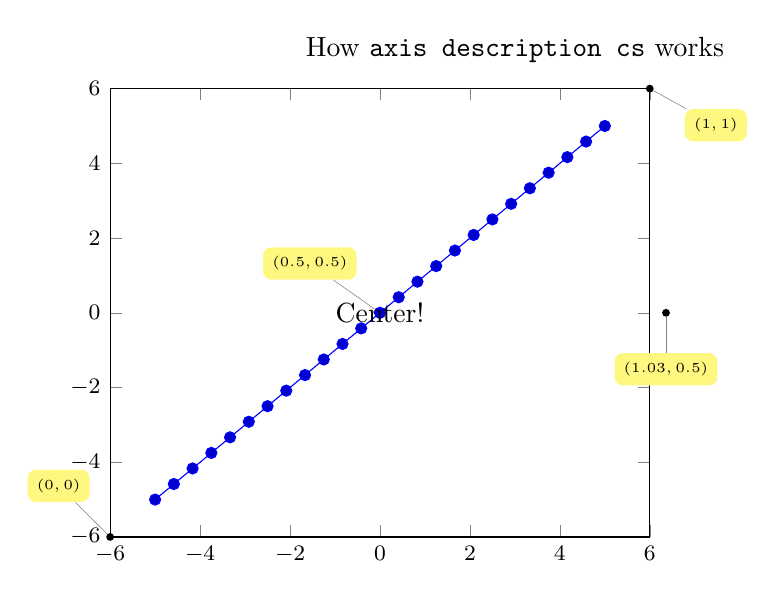
\begin{tikzpicture}
	\tikzset{
		every pin/.style={fill=yellow!50!white,rectangle,rounded corners=3pt,font=\tiny},
		small dot/.style={fill=black,circle,scale=0.3}
	}
	\begin{axis}[
		clip=false,
		title=How \texttt{axis description cs} works
	]
	\addplot {x};

	\node[small dot,pin=120:{$(0,0)$}]      at (axis description cs:0,0) {};
	\node[small dot,pin=-30:{$(1,1)$}]      at (axis description cs:1,1) {};
	\node[small dot,pin=-90:{$(1.03,0.5)$}] at (axis description cs:1.03,0.5) {};
	\node[small dot,pin=125:{$(0.5,0.5)$}]  at (axis description cs:0.5,0.5) {};
	\end{axis}
\end{tikzpicture}
\end{codeexample}

Axis descriptions are \Tikz\ nodes, that means all placement and detail options of \cite{tikz} apply. The point on the node's boundary which is actually shifted to the |at| coordinate needs to be provided with an anchor (cf~\cite[Nodes and Edges]{tikz}):
\begin{codeexample}[]
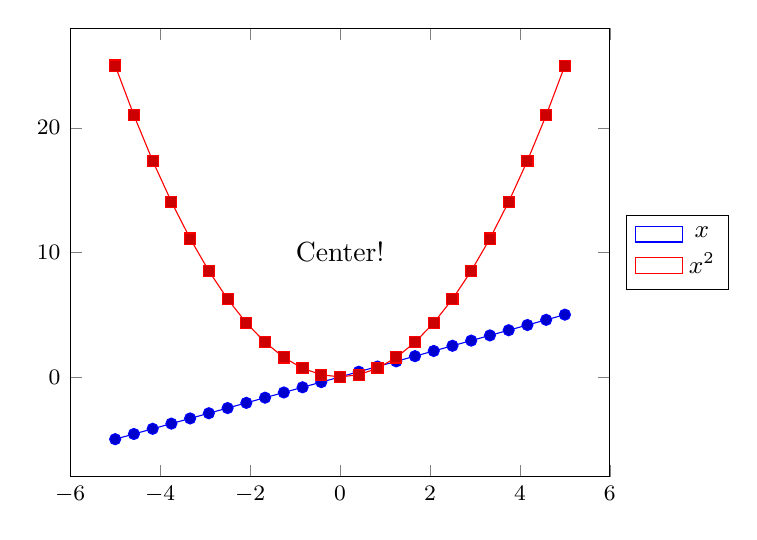
\begin{tikzpicture}
	\begin{axis}[
		legend entries={$x$,$x^2$},
		legend style={
			at={(1.03,0.5)},
			anchor=west
		}
	]
	\addplot {x};
	\addplot {x^2};
	\end{axis}
\end{tikzpicture}
\end{codeexample}
	
	Standard anchors of nodes are |north|, |east|, |south|, |west| and mixed components like |north east|.
	Please refer to \cite{tikz} for a complete documentation of anchors.

\paragraph{Remarks:} 
\begin{itemize}
	\item Each of the anchors described in section~\ref{pgfplots:sec:align} can be described by |axis description cs| as well.
	\item The |axis description cs| is independend of axis reversals or skewed axes.
	Only for the default configuration of boxed axes is it the same as |rel axis cs|, i.e.\ |(0,0)| is the same as the smallest axis coordinate and |(1,1)| is the largest one in case of standard boxed axes\footnote{This was different in versions before 1.3: earlier versions did not have the distinction between \texttt{axis description cs} and \texttt{rel axis cs}.}.

	\item Even for three dimensional axes, the |axis description cs| is still two-dimensional: it always refers to coordinates relative to the tightest bounding box around the axis (without any descriptions or ticks).
\begin{codeexample}[width=4cm]
% the same as above for 3D ...
% [See the TikZ manual if you'd like to learn about nodes and pins]
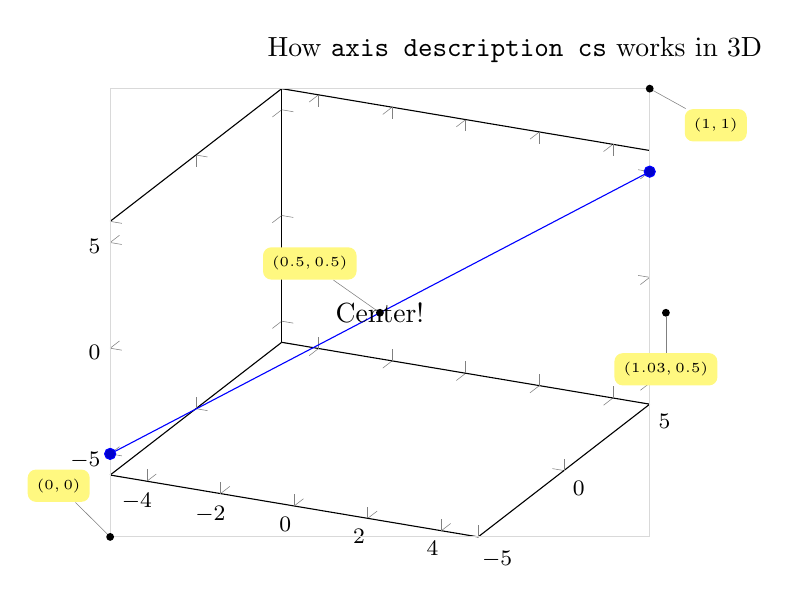
\begin{tikzpicture}
	\tikzset{
		every pin/.style={fill=yellow!50!white,rectangle,rounded corners=3pt,font=\tiny},
		small dot/.style={fill=black,circle,scale=0.3}
	}
	\begin{axis}[
		clip=false,
		title=How \texttt{axis description cs} works in 3D
	]
	\addplot3 coordinates {(-5,-5,-5) (5,5,5)};

	\draw[black!15] (axis description cs:0,0) rectangle (axis description cs:1,1);

	\node[small dot,pin=120:{$(0,0)$}]      at (axis description cs:0,0) {};
	\node[small dot,pin=-30:{$(1,1)$}]      at (axis description cs:1,1) {};
	\node[small dot,pin=-90:{$(1.03,0.5)$}] at (axis description cs:1.03,0.5) {};
	\node[small dot,pin=125:{$(0.5,0.5)$}]  at (axis description cs:0.5,0.5) {};
	\end{axis}
\end{tikzpicture}
\end{codeexample}
	
	\item Since the view does not influence these positions, |axis description cs| might not be a good choice for axis labels in 3D. The |ticklabel cs| is used in this case.
\end{itemize}
\end{coordinatesystem}

\begin{coordinatesystemlist}{%
	xticklabel cs,%
	yticklabel cs,%
	zticklabel cs,
	ticklabel cs}
	A set of special coordinate systems intended to place axis descriptions (or any other drawing operation) besides tick labels, in a way such that tick label are not obscured.

	See also |xlabel near ticks| as one main application of |ticklabel cs|.

	The |xticklabel cs| (and its variants) always refer to one, uniquely identified axis: the one which is (or would be) annotated with tick labels. The |ticklabel cs| can only be used in contexts where the axis is clear (for example, inside of |xlabel style| -- there, the |ticklabel cs| is equivalent to |xticklabel cs|).

	Each of these coordinate systems allows to specify points on a straight line which is placed parallel to an axis containing tick labels, moved away just far enough to avoid overlaps with the tick labels:
\begin{codeexample}[width=4cm]
\tikzset{
	every pin/.style={fill=yellow!50!white,rectangle,rounded corners=3pt,font=\tiny},
	small dot/.style={fill=black,circle,scale=0.3}
}
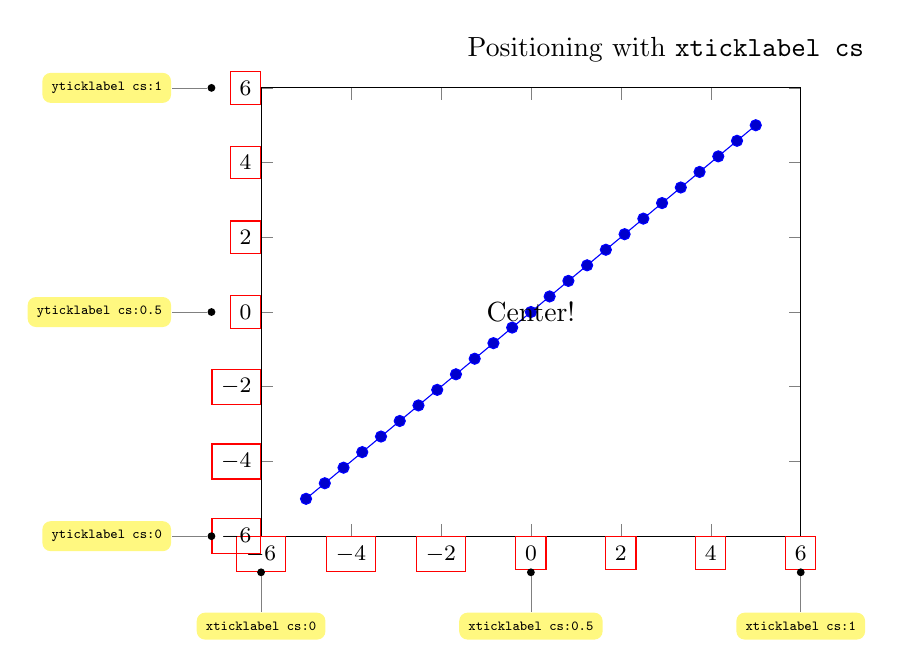
\begin{tikzpicture}
\begin{axis}[
	clip=false,
	ticklabel style={draw=red},
	title=Positioning with \texttt{xticklabel cs}]
	\addplot {x};
	\node[small dot,pin=-90:{\texttt{xticklabel cs:0}}]     at (xticklabel cs:0) {};
	\node[small dot,pin=-90:{\texttt{xticklabel cs:0.5}}]   at (xticklabel cs:0.5) {};
	\node[small dot,pin=-90:{\texttt{xticklabel cs:1}}]     at (xticklabel cs:1) {};


	\node[small dot,pin=180:{\texttt{yticklabel cs:0}}]     at (yticklabel cs:0) {};
	\node[small dot,pin=180:{\texttt{yticklabel cs:0.5}}]   at (yticklabel cs:0.5) {};
	\node[small dot,pin=180:{\texttt{yticklabel cs:1}}]     at (yticklabel cs:1) {};
\end{axis}
\end{tikzpicture}
\end{codeexample}

The basic idea is to place coordinates on a straight line which is parallel to the axis containing tick labels -- but shifted such that the line does not cut through tick labels.

Of course, it is relatively simple to get the same coordinates as in the two dimensional example above with |axis description cs|, except that |ticklabel cs| always respects the tick label sizes appropriately. However, |ticklabel cs| becomes far superior when it comes to three dimensional positioning:

\begin{codeexample}[width=4cm]
% the same as above for 3D ...
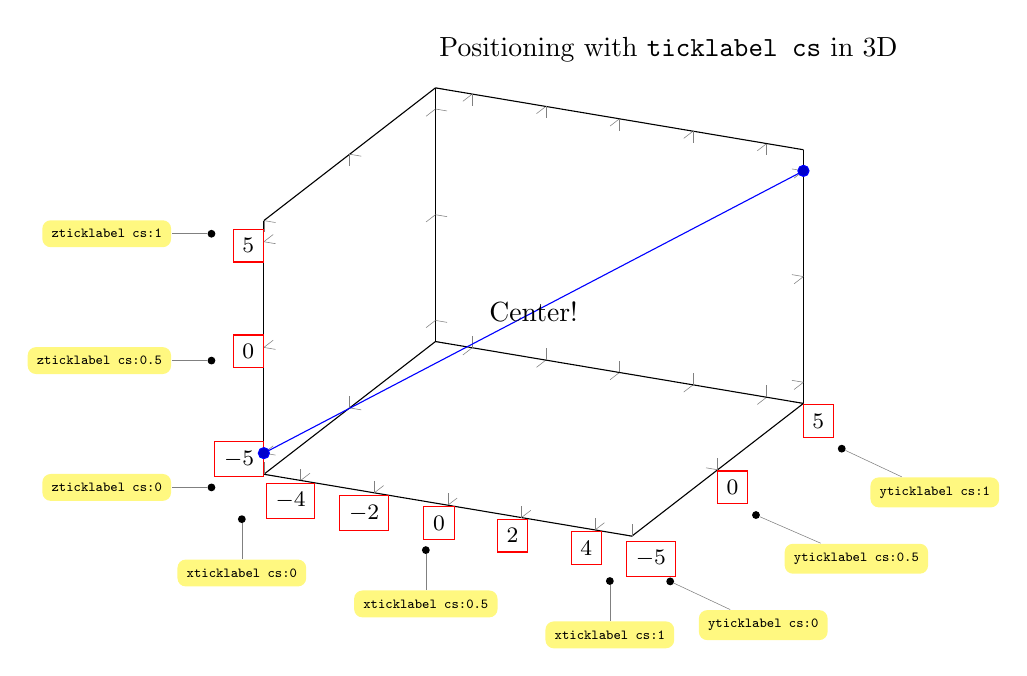
\begin{tikzpicture}
	\tikzset{
		every pin/.style={fill=yellow!50!white,rectangle,rounded corners=3pt,font=\tiny},
		small dot/.style={fill=black,circle,scale=0.3}
	}
	\begin{axis}[
		ticklabel style={draw=red},
		clip=false,
		title=Positioning with \texttt{ticklabel cs} in 3D
	]
	\addplot3 coordinates {(-5,-5,-5) (5,5,5)};

	\node[small dot,pin=-90:{\texttt{xticklabel cs:0}}]     at (xticklabel cs:0) {};
	\node[small dot,pin=-90:{\texttt{xticklabel cs:0.5}}]   at (xticklabel cs:0.5) {};
	\node[small dot,pin=-90:{\texttt{xticklabel cs:1}}]     at (xticklabel cs:1) {};

	\node[small dot,pin=-45:{\texttt{yticklabel cs:0}}]     at (yticklabel cs:0) {};
	\node[small dot,pin=-45:{\texttt{yticklabel cs:0.5}}]   at (yticklabel cs:0.5) {};
	\node[small dot,pin=-45:{\texttt{yticklabel cs:1}}]     at (yticklabel cs:1) {};

	\node[small dot,pin=180:{\texttt{zticklabel cs:0}}]     at (zticklabel cs:0) {};
	\node[small dot,pin=180:{\texttt{zticklabel cs:0.5}}]   at (zticklabel cs:0.5) {};
	\node[small dot,pin=180:{\texttt{zticklabel cs:1}}]     at (zticklabel cs:1) {};
	\end{axis}
\end{tikzpicture}
\end{codeexample}

	The coordinate |ticklabel cs:0| is associated to the lower axis limit while |ticklabel cs:1| is near the upper axis limit.  The value |0.5| is in the middle of the axis, any other values (including negative values or values beyond $1$) are linearly interpolated inbetween.

	The |ticklabel cs| also accepts a second (optional) argument: a shift ``away'' from the tick labels. The shift points to a vector which is orthogonal to the associated axis, away from the tick labels. A shift of |0pt| is directly at the edge of the tick labels in direction of the normal vector, positive values move the position away and negative closer to the tick labels.
\begin{codeexample}[width=4cm]
\tikzset{
	every pin/.style={fill=yellow!50!white,rectangle,rounded corners=3pt,font=\tiny},
	small dot/.style={fill=black,circle,scale=0.3}
}
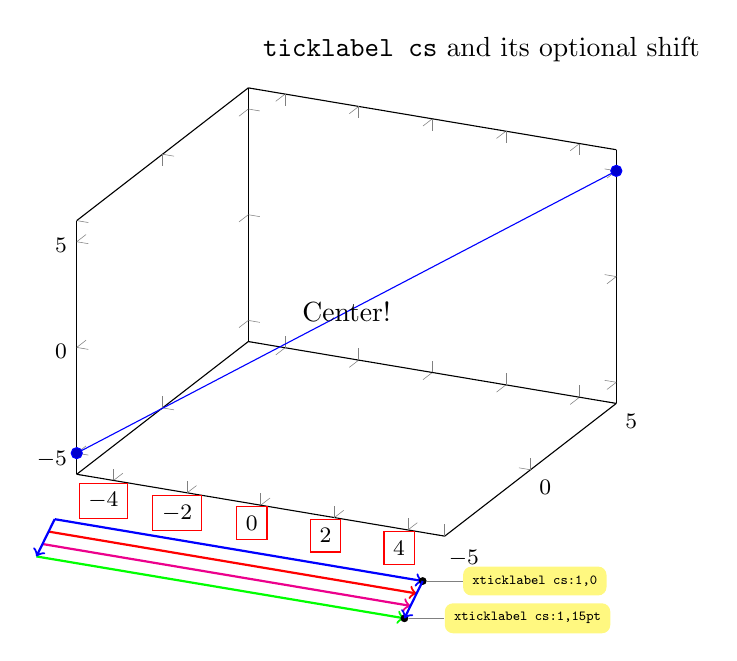
\begin{tikzpicture}
	\begin{axis}[
		xticklabel style={draw=red},
		clip=false,
		title=\texttt{ticklabel cs} and its optional shift
	]
	\addplot3 coordinates {(-5,-5,-5) (5,5,5)};

	\draw[blue,thick,->]      (xticklabel cs:0,0)     -- (xticklabel cs:1,0);
	\draw[red,thick,->]       (xticklabel cs:0,5pt)   -- (xticklabel cs:1,5pt);
	\draw[magenta,thick,->]   (xticklabel cs:0,10pt)  -- (xticklabel cs:1,10pt);
	\draw[green,thick,->]     (xticklabel cs:0,15pt)  -- (xticklabel cs:1,15pt);
	\node[small dot,pin=0:{\texttt{xticklabel cs:1,0}}]      at (xticklabel cs:1,0) {};
	\node[small dot,pin=0:{\texttt{xticklabel cs:1,15pt}}]   at (xticklabel cs:1,15pt) {};

	\draw[blue,thick,->]      (xticklabel cs:0,0)     -- (xticklabel cs:0,15pt);
	\draw[blue,thick,->]      (xticklabel cs:1,0)     -- (xticklabel cs:1,15pt);
	\end{axis}
\end{tikzpicture}
\end{codeexample}

	Whenever the |ticklabel cs| is used, the anchor should be set to |anchor=near ticklabel| (see below).

	There is one speciality: if you reverse an axis (with |x dir=reverse|), points provided by |ticklabel cs| will be \emph{unaffected} by the axis reversal. This is intented to provide consistent placement even for reversed axes. Use |allow reversal of rel axis cs=false| to disable this feature.
\end{coordinatesystemlist}


Axis descriptions can also be placed using the predefined node |current axis|. At the time when axis descriptions are drawn, all anchors which refer to the axis origin (that means the ``real'' point $(0,0)$) or any of the axis corners can be referenced using |current axis.|\meta{anchor name}. Please see section~\ref{pgfplots:sec:align}, Alignment, for further details.

\subsubsection{Alignment of Axis Descriptions}
This section describes how to modify the default alignment of axis descriptions. It can be skipped at first reading.

The two topics positioning and alignment always work together: \emph{positioning} means to select an appropriate coordinate and \emph{alignment} means to select an anchor inside of the description which will actually be moved to the desired position.

\Tikz\ uses many anchors to provide alignment; most of them are named like |north|, |north east| etc. These names hold for any axis description as well (as axis description are \Tikz\ nodes). Readers can learn details about this topic in the \Tikz\ manual~\cite{tikz} or some more advice in section~\ref{pgfplots:sec:align}.

When it comes to axis descriptions, \PGFPlots\ offers some specialized anchors and alignment methods which are described below.
\begin{anchorlist}{near xticklabel,near yticklabel,near zticklabel,near ticklabel}
	These anchors can be used to align at the part of an axis description which is nearest to the tick labels of a particular axis.

	These anchors are used for axis labels, especially for three dimensional axes.

\label{key:near:ticklabel}
	Maybe it is best to demonstrate it by example:
\begin{codeexample}[]
\begin{tikzpicture}
	\begin{axis}[
		title=Without \texttt{near ticklabel},
		ylabel={$f(x)=x$},
		every axis y label/.style=
			{at={(ticklabel cs:0.5)},rotate=90,anchor=center},
		clip=false,% to display the \path below
		ylabel style={draw=red},
		yticklabel style={draw=red}
	]

		\addplot {x};

		% visualize the position:
		\fill (yticklabel cs:0.5) circle(2pt);
	\end{axis}
\end{tikzpicture}%
~
\begin{tikzpicture}
	\begin{axis}[
		title=With \texttt{near ticklabel},
		ylabel={$f(x)=x$},
		every axis y label/.style=
			{at={(ticklabel cs:0.5)},rotate=90,anchor=near ticklabel},
		clip=false,
		ylabel style={draw=red},
		yticklabel style={draw=red}
	]

		\addplot {x};
		\fill (yticklabel cs:0.5) circle(2pt);
	\end{axis}
\end{tikzpicture}
\end{codeexample}

	The motivation is to place nodes such that they are anchored next to the tick label, regardless of the node's rotation or the position of ticks. The special anchor |near ticklabel| is only available for axis labels (as they have a uniquely identified axis, either $x$, $y$ or $z$).

	In more detail, the anchor is placed such on the intersection of the node's shape with the outer normal vector of the tick label axis. This normal vector is the same which is used for the shift argument in |ticklabel cs|: it is orthogonal to the tick label axis. Furthermore, |near ticklabel| inverts the transformation matrix before it computes this intersection point.

	The |near ticklabel| anchor and its friends will be added temporarily to any shape used for an axis description.
\end{anchorlist}

\begin{pgfplotsxykeylist}{/tikz/sloped like \x\space axis}
	A key which replaces the rotational / scaling parts of the transformation matrix such that the node is sloped like the provided axis. For two dimensional plots, |sloped like y axis| is effectively the same as |rotate=90|. For a three dimensional axis, this will lead to a larger difference:
\pgfplotsexpensiveexample
\begin{codeexample}[]
\begin{tikzpicture}
	\begin{axis}[
		xlabel=Variable 1,
		ylabel=Variable 2,
		zlabel=value,
		xlabel style={sloped like x axis},
		ylabel style={sloped}
	]

	\addplot3[surf] {y*x*(1-x)};
	\end{axis}
\end{tikzpicture}
\end{codeexample}

	Inside of axis labels, |sloped| is an alias |sloped like |\meta{char}| axis| with the correct \meta{char} chosen automatically.

	Please note that rotated text might not look very good (neither on screen nor printed).
\end{pgfplotsxykeylist}


\subsubsection{Labels}

\begin{pgfplotsxykey}{\x label=\marg{text}}
The options |xlabel| and |ylabel| change axis labels to \marg{text} which is any \TeX\ text. Use curly braces to include special characters, for example ``|xlabel={, = characters}|'' if characters like `|=|' or `|,|' need to be included literally.

Labels are \Tikz-Nodes which are placed with
\begin{codeexample}[code only]
% for x:
\node 
	[style=every axis label,
	style=every axis x label]

% for y:
\node 
	[style=every axis label,
	style=every axis y label] 
\end{codeexample}
so their position and appearance can be customized. 

The label placement has been modified in version 1.3, since the new |ticklabel cs| allows to respect the size of adjacent tick label sizes. To maintain backwards compatibility, version 1.3 supports a new-feature switch and uses the same, sub-optimal initial settings as versions before 1.3:

\begin{pgfplotsxykeylist}{\x label shift=\marg{dimension} (initially 0pt),label shift=\marg{dimension}}
	Shifts labels in direction of the outer normal vector of the axis by an amount of \marg{dimension}. The |label shift| sets all three label shifts to the same value.

	\paragraph{Attention:} This does only work if |\pgfplotsset{compat=newest}| has been called (More precisely: if |xlabel near ticks| is active for the respective axis).
\end{pgfplotsxykeylist}

\begin{pgfplotsxykeylist}{\x label near ticks,compat=newest}
	These keys place axis labels (those of |xlabel|) near the tick labels. If tick labels are small, labels will move closer to the axis. If tick labels are large, axis labels will move away from the axis. This is the default for every three dimensional plot, but it \emph{won't} be used initially for two--dimensional plots for backwards compatibility. Take a look at the definition of |near ticklabel| on page~\pageref{key:near:ticklabel} for an example.

	The definition of these styles is
\begin{codeexample}[code only]
\pgfplotsset{
	/pgfplots/xlabel near ticks/.style={
		/pgfplots/every axis x label/.style={at={(ticklabel cs:0.5)},anchor=near ticklabel}
	},
	/pgfplots/ylabel near ticks/.style={
		/pgfplots/every axis y label/.style={at={(ticklabel cs:0.5)},rotate=90,anchor=near ticklabel}
	}
}
\end{codeexample}
	
	It is encouraged to write
\begin{codeexample}[code only]
\pgfplotsset{compat=newest}
\end{codeexample}
	\noindent in your preamble to install the styles document-wide -- it leads to the best output (it avoids unnecessary space). It is not activated initially for backwards compatibility with older versions which used fixed distances from the tick labels.
\end{pgfplotsxykeylist}

\begin{pgfplotsxykeylist}{\x label absolute,compat=pre 1.3}
	Installs placement styles for axis labels such that |xlabel| yields a description of absolute, fixed distance to the axis. This is the initial configuration (for backwards compatibility with versions before 1.3). Use |compat=newest| to get the most recent, more flexible configuration. Take a look at the definition of |near ticklabel| on page~\pageref{key:near:ticklabel} for an example.

	These styles are defined by
\begin{codeexample}[code only]
\pgfplotsset{
	/pgfplots/xlabel absolute/.style={%
		/pgfplots/every axis x label/.style={at={(0.5,0)},below,yshift=-15pt},%
		/pgfplots/every x tick scale label/.style={at={(1,0)},yshift=-2em,left,inner sep=0pt},
	},
	/pgfplots/ylabel absolute/.style={%
		/pgfplots/every axis y label/.style={at={(0,0.5)},xshift=-35pt,rotate=90},
		/pgfplots/every y tick scale label/.style={at={(0,1)},above right,inner sep=0pt,yshift=0.3em},
	}
}
\end{codeexample}

	There is no predefined absolute placement style for three dimensional axes.
\end{pgfplotsxykeylist}

Whenever possible, consider using |/.append style| instead of overwriting the default styles to ensure compatibility with future versions.
\begin{codeexample}[code only]
\pgfplotsset{every axis label/.append style={...}}
\pgfplotsset{every axis x label/.append style={...}}
\pgfplotsset{every axis y label/.append style={...}}
\end{codeexample}
	Use |xlabel/.add=|\marg{prefix}\marg{suffix} to modify an already assigned label.
\end{pgfplotsxykey}

\begin{pgfplotskey}{title=\marg{text}}
Adds a caption to the plot. This will place a \Tikz-Node with
\begin{codeexample}[code only]
\node[style=every axis title] {text};
\end{codeexample}
to the current axis.
\begin{codeexample}[]
\begin{tikzpicture}
\begin{loglogaxis}[
	xlabel=Dof,ylabel=Error,
	title={$\mu=0.1$, $\sigma=0.2$}]

	\addplot coordinates {
		(5,    8.312e-02)
		(17,   2.547e-02)
		(49,   7.407e-03)
		(129,  2.102e-03)
		(321,  5.874e-04)
		(769,  1.623e-04)
		(1793, 4.442e-05)
		(4097, 1.207e-05)
		(9217, 3.261e-06)
	};
\end{loglogaxis}
\end{tikzpicture}%
\end{codeexample}
%--------------------------------------------------
% \hfill
% \begin{tikzpicture}
% \begin{loglogaxis}[
% 	width=0.48\linewidth,
% 	xlabel=Dof,ylabel=Error,
% 	title={$\mu=1$, $\sigma=\frac{1}{2}$}]
% 
% 	\addplot[color=red,mark=*] coordinates {
% 		(7,		8.472e-02)
% 		(31,	3.044e-02)
% 		(111,	1.022e-02)
% 		(351,	3.303e-03)
% 		(1023,	1.039e-03)
% 		(2815,	3.196e-04)
% 		(7423,	9.658e-05)
% 		(18943,	2.873e-05)
% 		(47103,	8.437e-06)
% 	};
% \end{loglogaxis}
% \end{tikzpicture}
%-------------------------------------------------- 
The title's appearance and/or placing can be reconfigured with
\begin{codeexample}[code only]
\pgfplotsset{every axis title/.append style={at={(0.75,1)}}}
\end{codeexample}
This will place the title at~75\% of the $x$-axis. The coordinate~$(0,0)$ is the lower left corner and~$(1,1)$ the upper right one.

Use |title/.add=|\marg{prefix}\marg{suffix} to modify an already assigned title.
\end{pgfplotskey}

\begin{pgfplotscodekey}{extra description}
Allows to insert \marg{commands} after axis labels, titles and legends have been typeset.

As all other axis descriptions, the code can use $(0,0)$ to access the lower left corner and $(1,1)$ to access the upper right one. It won't be clipped.
\begin{codeexample}[]
\pgfplotsset{every axis/.append style={
	extra description/.code={
		\node at (0.5,0.5) {Center!};
	}}}
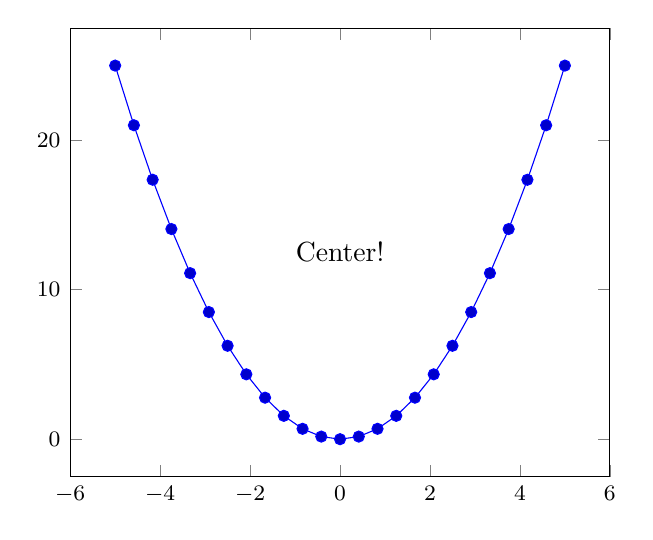
\begin{tikzpicture}
	\begin{axis}
	\addplot {x^2};
	\end{axis}
\end{tikzpicture}
\end{codeexample}
\end{pgfplotscodekey}


\subsubsection{Legends}
\label{pgfplots:sec:legendopts}
\label{pgfplots:sec:legendcmds}
Legends can be generated in two ways: the first is to use |\addlegendentry| or |\legend| inside of an axis. The other method is to use the key |legend entries|.


\begin{command}{\addlegendentry\marg{name}}
Adds a single legend entry to the legend list. This will also enable legend drawing.
\begin{codeexample}[]
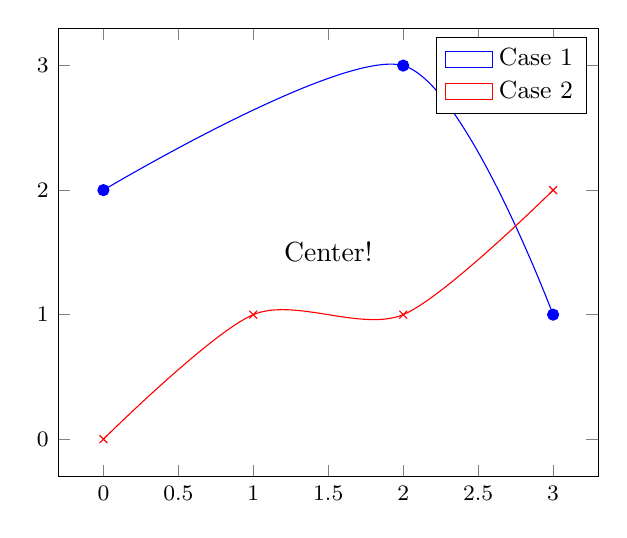
\begin{tikzpicture}
\begin{axis}
\addplot[smooth,mark=*,blue] coordinates {
	(0,2)
	(2,3)
	(3,1)
};
\addlegendentry{Case 1}

\addplot[smooth,color=red,mark=x]
	coordinates {
		(0,0)
		(1,1)
		(2,1)
		(3,2)
	};
\addlegendentry{Case 2}
\end{axis}
\end{tikzpicture}
\end{codeexample}
It does not matter where |\addlegendentry| commands are placed, only the sequence matters. You will need one |\addlegendentry| for every |\addplot| command (unless you prefer an empty legend).


Using |\addlegendentry| disables the key |legend entries|.
\end{command}

\begin{command}{\addlegendentryexpanded\marg{\TeX\ text}}
	A variant of |\addlegendentry| which provides a method to deal with macros inside of \meta{\TeX\ text}.

	Suppose \meta{\TeX\ text} contains some sort of parameter which varies \emph{for every plot}. Moreover, you like to use a loop to generate the plots. Then, it is simpler to use |\addlegendentryexpanded|:
\begin{codeexample}[]
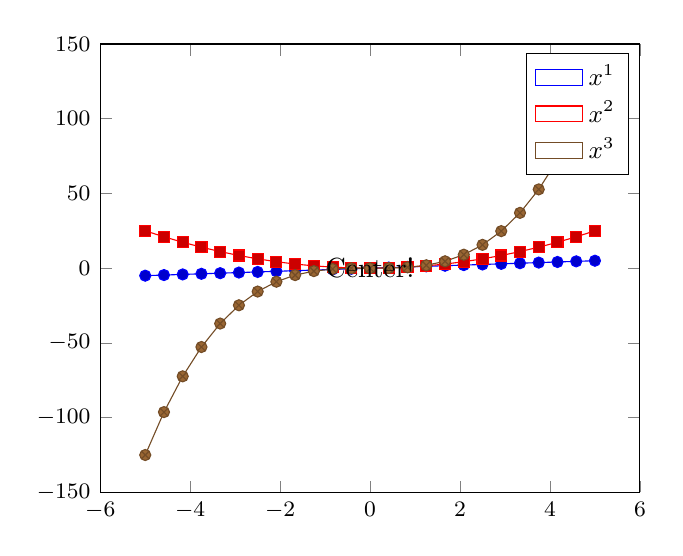
\begin{tikzpicture}
\begin{axis}
	\foreach \p in {1,2,3} {
		\addplot {x^\p};
		\addlegendentryexpanded{$x^\p$}
	}
\end{axis}
\end{tikzpicture}
\end{codeexample}
	Note that this example wouldn't have worked with |\addlegendentry{$x^\p$}| because the macro |\p| is no longer defined when \PGFPlots\ attempts to draw the legend.

	The invocation of |\addlegendentryexpanded{$x^\p$}| is equivalent to calling |\addlegendentry{$x^2$}| if |\p| expands to |2|.

	The argument \meta{\TeX\ text} is expanded until nothing but un-expandable material remains (i.e.\ it uses the \TeX\ primitive |\edef|). Occasionally, \marg{\TeX\ text} contains parts which should be expanded (like |\p|) and other parts which should be left unexpanded (for example |\pgfmathprintnumber{\p}|). Then, use
	
		|\noexpand\pgfmathprintnumber{\p}|
	
	or, equivalently

		|\protect\pgfmathprintnumber{\p}|

	to avoid expansion of the macro which follows the |\protect| immediately.
\end{command}



\begin{command}{\legend\marg{list}}
\label{sec:legenddef}%
You can use |\legend|\marg{list} to assign a complete legend.
\begin{codeexample}[code only]
\legend{$d=2$,$d=3$,$d=4$,$d=5$,$d=6$}
\end{codeexample}
The argument of |\legend| is a comma--separated list of entries, one for each plot. It is processed using the \PGF\ |\foreach| command\footnote{Older versions of \PGFPlots\ used \texttt{\textbackslash legend\{first\textbackslash\textbackslash second\textbackslash\textbackslash third\textbackslash\textbackslash\}} instead of comma--separated lists. This syntax is still accepted.}.
The short marker/line combination shown in legends is acquired from the \marg{style options} argument of |\addplot|.

Using |\legend| overwrites any other existing legend entries.
\end{command}


\begin{pgfplotskey}{legend entries=\marg{comma separated list}}
	This key can be used to assign legend entries just like the commands |\addlegendentry| and |\legend|. Again, the positioning is relative to the axis rectangle (unless units like |cm| or |pt| are specified explicitly).
\begin{codeexample}[]
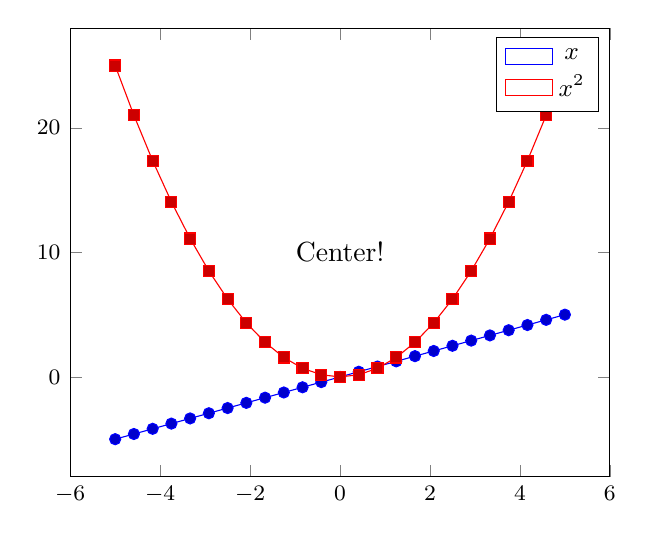
\begin{tikzpicture}
	\begin{axis}[legend entries={$x$,$x^2$}]
	\addplot {x};
	\addplot {x^2};
	\end{axis}
\end{tikzpicture}
\end{codeexample}

	The commands for legend creation take precedence: the key |legend entries| is only considered if there is no legend command in the current axis. 
\begin{codeexample}[]
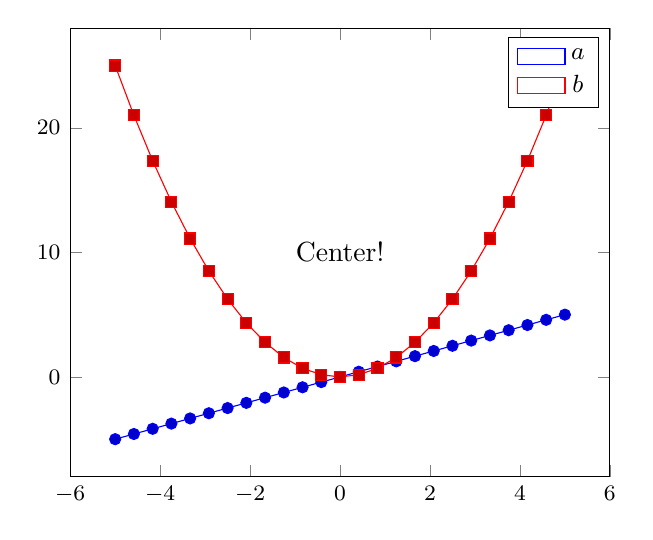
\begin{tikzpicture}
	\begin{axis}[legend entries={$x$,$x^2$}]
	\addplot {x};
	\addplot {x^2};
	\legend{$a$,$b$}% overrides the option
	\end{axis}
\end{tikzpicture}
\end{codeexample}
	Please be careful with whitespaces in \marg{comma separated list}: they will contribute to legend entries. Consider using `|%|' at the end of each line in multiline arguments (the end of line character is also a whitespace in \TeX).
\end{pgfplotskey}


\subsubsection{Legend Appearance}

{%
\pgfplotsset{every axis/.append style={width=3cm,scale only axis,legend style={font=\footnotesize}}}%


\begin{stylekey}{/pgfplots/every axis legend}
The style ``|every axis legend|'' determines the legend's position and outer appearance:
\begin{codeexample}[code only]
\pgfplotsset{every axis legend/.append style={
		at={(0,0)},
		anchor=south west}}
\end{codeexample}
will draw it at the lower left corner of the axis while
\begin{codeexample}[code only]
\pgfplotsset{every axis legend/.append style={
		at={(1,1)},
		anchor=north east}}
\end{codeexample}
means the upper right corner. The `|anchor|' option determines which point \emph{of the legend} will be placed at $(0,0)$ or $(1,1)$.

The legend is a \Tikz-matrix, so one can use any \Tikz\ option which affects
nodes and matrizes (see~\cite[section 13~and~14]{tikz}). The matrix is created by something like
\begin{codeexample}[code only]
\matrix[style=every axis legend] {
	draw plot specification 1 & \node{legend 1}\\
	draw plot specification 2 & \node{legend 2}\\
	...
};
\end{codeexample}

\begin{codeexample}[]
\pgfplotsset{every axis legend/.append style={
		at={(1.02,1)},
		anchor=north west}}
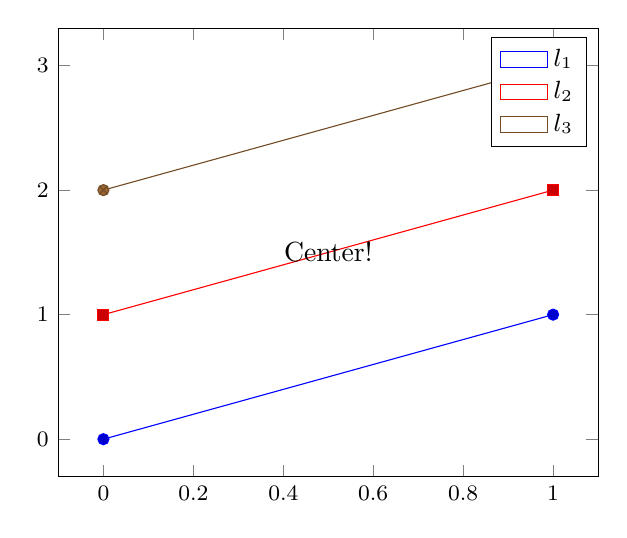
\begin{tikzpicture}
\begin{axis}
\addplot coordinates {(0,0) (1,1)};
\addplot coordinates {(0,1) (1,2)};
\addplot coordinates {(0,2) (1,3)};
\legend{$l_1$,$l_2$,$l_3$}
\end{axis}
\end{tikzpicture}
\end{codeexample}

Use |legend columns=|\marg{number} to configure the number of horizontal legend entries.
\begin{codeexample}[]
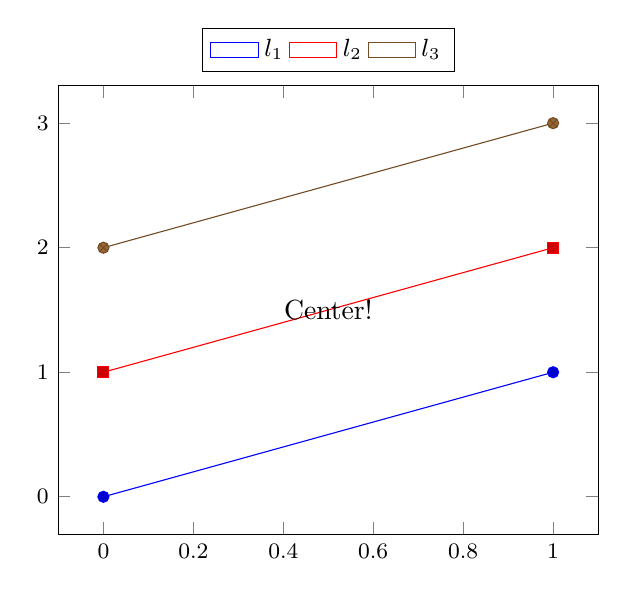
\begin{tikzpicture}
\pgfplotsset{every axis legend/.append style={
		at={(0.5,1.03)},
		anchor=south}}
\begin{axis}[legend columns=4]
\addplot coordinates {(0,0) (1,1)};
\addplot coordinates {(0,1) (1,2)};
\addplot coordinates {(0,2) (1,3)};
\legend{$l_1$,$l_2$,$l_3$}
\end{axis}
\end{tikzpicture}
\end{codeexample}
\noindent
Instead of the |.append style|, it is possible to use |legend style| as in the following example. It has the same effect.

\begin{codeexample}[]
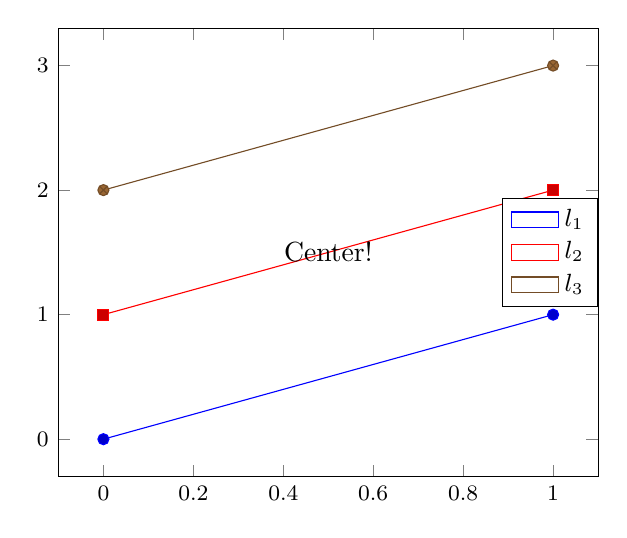
\begin{tikzpicture}
\begin{axis}[
	legend style={
		at={(1,0.5)},
		anchor=east}]
\addplot coordinates {(0,0) (1,1)};
\addplot coordinates {(0,1) (1,2)};
\addplot coordinates {(0,2) (1,3)};
\legend{$l_1$,$l_2$,$l_3$}
\end{axis}
\end{tikzpicture}
\end{codeexample}

\noindent
The default |every axis legend| style is
\begin{codeexample}[code only]
\pgfplotsset{every axis legend/.style={%
	cells={anchor=center},% Centered entries
	inner xsep=3pt,inner ysep=2pt,nodes={inner sep=2pt,text depth=0.15em},
	anchor=north east,%
	shape=rectangle,%
	fill=white,%
	draw=black,
	at={(0.98,0.98)}
}}
\end{codeexample}
Whenever possible, consider using |.append style| to keep the default styles active. This ensures compatibility with future versions.
\begin{codeexample}[code only]
\pgfplotsset{every axis legend/.append style={...}}
\end{codeexample}
\end{stylekey}

\pgfplotsshortstylekey legend style=every axis legend\pgfeov


\begin{pgfplotskey}{legend pos=\mchoice{south west,south east,north west,north east,outer north east}}
	A style which provides shorthand access to some commonly used legend positions.

	Each of these styles appends |at={(|\meta{x}|,|\meta{y}|)},anchor=|\meta{name} values to |every axis legend|.

\begin{codeexample}[]
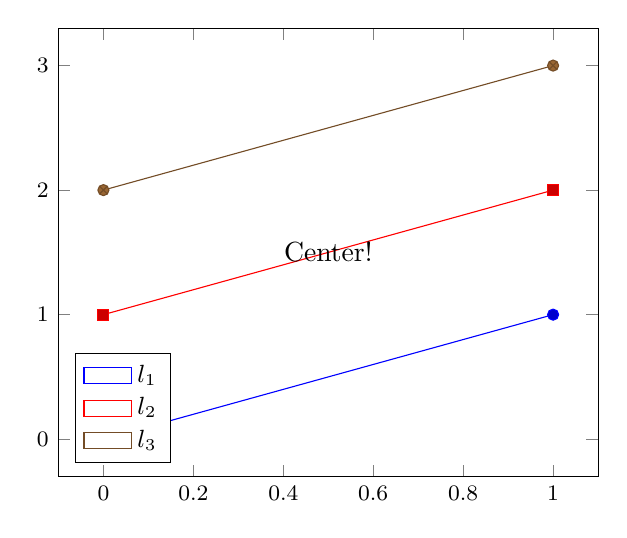
\begin{tikzpicture}
\begin{axis}[legend pos=south west]
\addplot coordinates {(0,0) (1,1)};
\addplot coordinates {(0,1) (1,2)};
\addplot coordinates {(0,2) (1,3)};
\legend{$l_1$,$l_2$,$l_3$}
\end{axis}
\end{tikzpicture}
\end{codeexample}

\begin{codeexample}[]
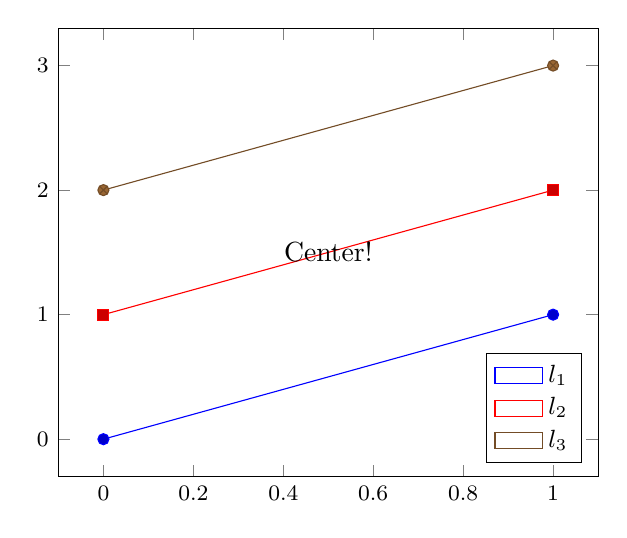
\begin{tikzpicture}
\begin{axis}[legend pos=south east]
\addplot coordinates {(0,0) (1,1)};
\addplot coordinates {(0,1) (1,2)};
\addplot coordinates {(0,2) (1,3)};
\legend{$l_1$,$l_2$,$l_3$}
\end{axis}
\end{tikzpicture}
\end{codeexample}

\begin{codeexample}[]
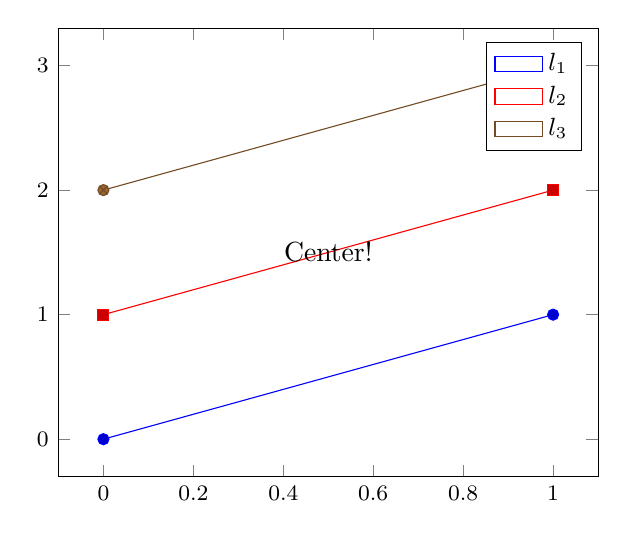
\begin{tikzpicture}
\begin{axis}[legend pos=north east]
\addplot coordinates {(0,0) (1,1)};
\addplot coordinates {(0,1) (1,2)};
\addplot coordinates {(0,2) (1,3)};
\legend{$l_1$,$l_2$,$l_3$}
\end{axis}
\end{tikzpicture}
\end{codeexample}

\begin{codeexample}[]
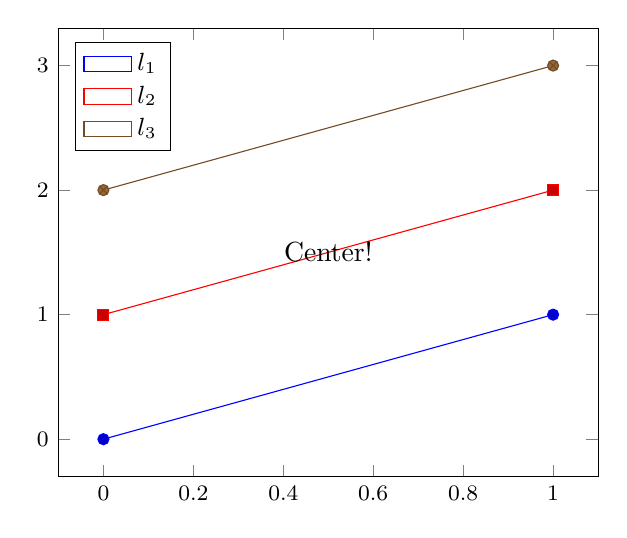
\begin{tikzpicture}
\begin{axis}[legend pos=north west]
\addplot coordinates {(0,0) (1,1)};
\addplot coordinates {(0,1) (1,2)};
\addplot coordinates {(0,2) (1,3)};
\legend{$l_1$,$l_2$,$l_3$}
\end{axis}
\end{tikzpicture}
\end{codeexample}

\begin{codeexample}[]
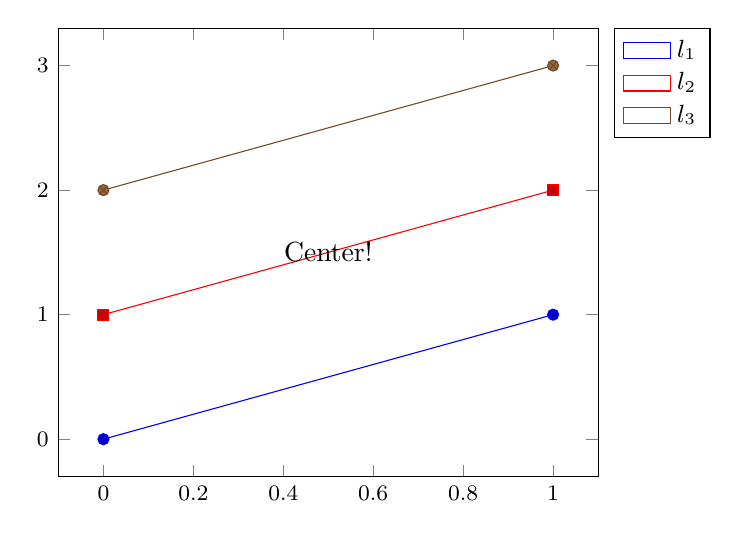
\begin{tikzpicture}
\begin{axis}[legend pos=outer north east]
\addplot coordinates {(0,0) (1,1)};
\addplot coordinates {(0,1) (1,2)};
\addplot coordinates {(0,2) (1,3)};
\legend{$l_1$,$l_2$,$l_3$}
\end{axis}
\end{tikzpicture}
\end{codeexample}
\end{pgfplotskey}

}

\begin{pgfplotskey}{legend columns=\marg{number} (default 1)}
Allows to configure the maximum number of adjacent legend entries. The default value~|1| places legend entries vertically below each other. 

Use |legend columns=-1| to draw all entries horizontally.
\end{pgfplotskey}

\begin{pgfplotskey}{legend plot pos=\mchoice{left,right,none} (initially left)}
Configures where the small line specifications will be drawn: left of the description, right of the description or not at all.
\end{pgfplotskey}

\begin{pgfplotscodekey}{legend image code}
\label{opt:legend:image:code}
Allows to replace the default images which are drawn inside of legends. The first argument\footnote{As of version 1.3, this is no longer true -- now, the argument is empty and the plot specification is set \emph{before} \texttt{legend image code} is evaluated. This allows plot styles to change legend drawing commands.} to this option is the plot specification, a key-value list which has been determined by |\addplot|.

The default is
\begin{codeexample}[code only]
/pgfplots/legend image code/.code={%
	\draw[mark repeat=2,mark phase=2,#1] 
		plot coordinates {
			(0cm,0cm) 
			(0.3cm,0cm)
			(0.6cm,0cm)%
		};%
}
\end{codeexample}
\end{pgfplotscodekey}

\begin{pgfplotskey}{reverse legend=\mchoice{true,false} (initially false)}
	Allows to reverse the order in which the pairs (legend entry, plot style) are drawn.
\begin{codeexample}[]
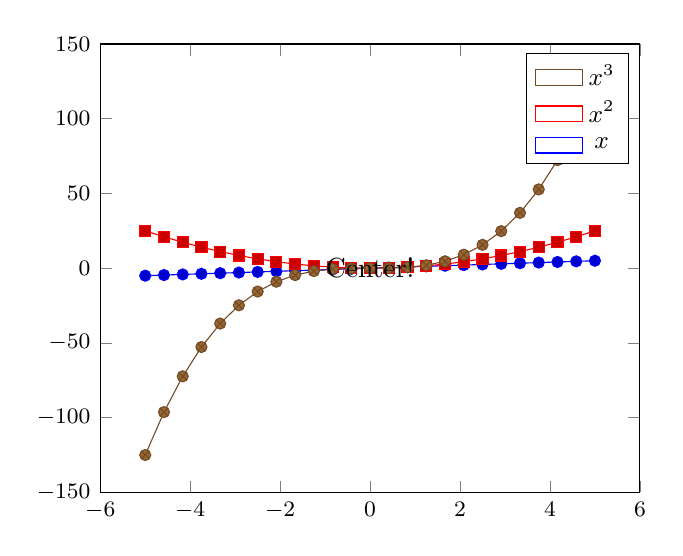
\begin{tikzpicture}
	\begin{axis}[reverse legend]
	\addplot {x};
	\addlegendentry{$x$}
	\addplot {x^2};
	\addlegendentry{$x^2$}
	\addplot {x^3};
	\addlegendentry{$x^3$}
	\end{axis}
\end{tikzpicture}
\end{codeexample}
\end{pgfplotskey}

\begin{stylekey}{/pgfplots/line legend}
	A style which sets |legend image code| back to its initial value. See the |legend image code| for the exact code. The purpose of this is mainly to
        be used in conjunction with the |area legend| key. See in the example under that key.
\begin{codeexample}[code only]
\pgfplotsset{
    legend image code/.code={%
	\draw[mark repeat=2,mark phase=2,#1] 
		plot coordinates {
			(0cm,0cm) 
			(0.3cm,0cm)
			(0.6cm,0cm)%
		};%
        }
}
\end{codeexample}
\end{stylekey}

\begin{stylekey}{/pgfplots/area legend}
	A style which sets |legend image code| to
\begin{codeexample}[code only]
\pgfplotsset{
	legend image code/.code={%
		\draw[#1] (0cm,-0.1cm) rectangle (0.6cm,0.1cm);
	}
}	
\end{codeexample}
	
% \usetikzlibrary{patterns}
\begin{codeexample}[]
% \usetikzlibrary{patterns}
\begin{tikzpicture}
\begin{axis}[area legend,
	axis x line=bottom,
	axis y line=left,
	domain=0:1,
	legend style={at={(0.03,0.97)},
		anchor=north west},
	axis on top,xmin=0]
\addplot[pattern=crosshatch dots,
	pattern color=blue,draw=blue,
	samples=500] 
	{sqrt(x)}	\closedcycle;

\addplot[pattern=crosshatch,
	pattern color=blue!30!white,
	draw=blue!30!white]
	{x^2} \closedcycle;

\addplot[red,line legend] coordinates {(0,0) (1,1)};
\legend{$\sqrt x$,$x^2$,$x$}
\end{axis}
\end{tikzpicture}
\end{codeexample}
\end{stylekey}

\subsubsection{Legends with \texttt{\textbackslash label} and \texttt{\textbackslash ref}}
\label{pgfplots:legend:labelref}
\PGFPlots\ offers a |\label| and |\ref| feature for \LaTeX\ to assemble a legend manually, for example as part of the figure caption. These references work as usual \LaTeX\ references: a |\label| remembers where and what needs to be referenced and a |\ref| expands to proper text. In context of plots, a |\label| remembers the plot specification of one plot and a |\ref| expands to the small image which would also be used inside of legends.
\begin{codeexample}[]
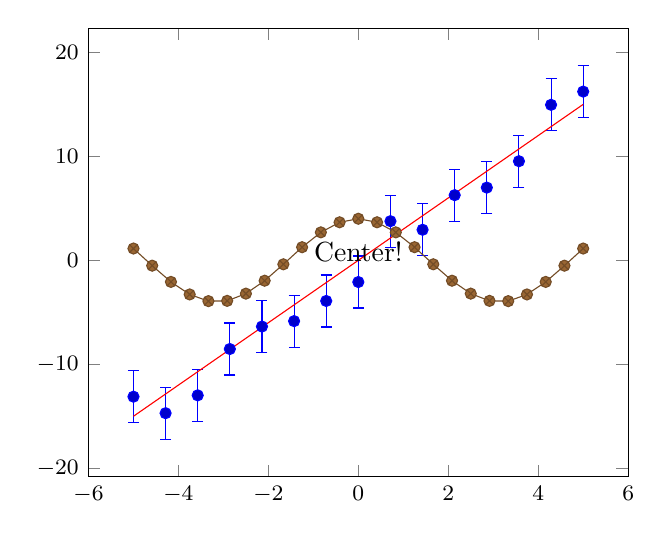
\begin{tikzpicture}[baseline]
\begin{axis}
	\addplot+[only marks,
			samples=15,
			error bars/y dir=both,
			error bars/y fixed=2.5]
		{3*x+2.5*rand};
	\label{pgfplots:label1}

	\addplot+[mark=none] {3*x};
	\label{pgfplots:label2}

	\addplot {4*cos(deg(x))};
	\label{pgfplots:label3}
\end{axis}
\end{tikzpicture}
\end{codeexample}
\begin{codeexample}[code only]
The picture shows the estimations \ref{pgfplots:label1} which are subjected to noise.
It appears the model \ref{pgfplots:label2} fits the data appropriately. 
Finally, \ref{pgfplots:label3} is only here to get three examples.
\end{codeexample}
\noindent The picture shows the estimations \ref{pgfplots:label1} which are subjected to noise.
It appears the model \ref{pgfplots:label2} fits the data appropriately. 
Finally, \ref{pgfplots:label3} is only here to get three examples.

\begin{commandlist}{\label\marg{label name},\label\oarg{reference}\marg{label name}}
	When used after |\addplot|, this command creates a \LaTeX\ label named \marg{label name}\footnote{This feature is \emph{only} available in \LaTeX, sorry.}. If this label is cross-referenced with |\ref|\marg{label name} somewhere, the associated plot specification will be inserted.
\begin{codeexample}[]
Label3 = \ref{pgfplots:label3}; 
Label2 = \ref{pgfplots:label2}
\end{codeexample}
	The label is assembled using |legend image code| and the plot style of the last plot. Any \PGFPlots\ option is expanded until only \Tikz\ (or \pgfname) options remain; these options are used to get an independant label\footnote{Please note that you can't use the label/ref mechanism in conjunction with image externalization as this will (naturally) lead to undefined references.}.

	More precisely, the small image generated by |\ref|\marg{label name} is 
\begin{codeexample}[code only]
\tikz[/pgfplots/every crossref picture] {...}
\end{codeexample}
	\noindent where the contents is determined by |legend image code| and the plot style.

	The second syntax, |\label|\oarg{reference}\marg{label name} allows to label particular pieces of an |\addplot| command. It is (currently) only interesting for |scatter/classes|: there,  it allows to reference particular classes of the scatter plot. See page~\pageref{pgfplots:scatterclasses} for more details.
\end{commandlist}

\begin{command}{\ref\marg{label name}}
	Can be used to reference a labeled, single plot. See the example above.

	This will also work together with |hyperref| links and |\pageref|\footnote{Older versions of \PGFPlots\ required the use of \texttt{\textbackslash protect\textbackslash ref} when used inside of captions or section headings. This is no longer necessary.}.
\end{command}

\begin{key}{/pgfplots/refstyle=\marg{label name}}
	Can be used to set the \emph{styles} of a labeled, single plot. This allows to write
\begin{codeexample}[code only]
\addplot[/pgfplots/refstyle={pgfplots:label2}]
\end{codeexample}
	\noindent somewhere. Please note that it may be easier to define a style with |.style|.
\end{key}

\begin{stylekey}{/pgfplots/every crossref picture}
	A style which will be used by the cross-referencing feature for plots. The default is
\begin{codeexample}[code only]
\pgfplotsset{every crossref picture/.style={baseline,yshift=0.3em}}
\end{codeexample}
\end{stylekey}

\subsubsection{Axis Lines}
By default the axis lines are drawn as a |box|, but it is possible to change the appearance of the $x$~and~$y$ axis lines.

\begin{pgfplotskeylist}{
	axis x line=\mchoice{box,top,middle,center,bottom,none} (initially box),
	axis x line*=\mchoice{box,top,middle,center,bottom,none} (initially box),
	axis y line=\mchoice{box,left,middle,center,right,none} (initially box),
	axis y line*=\mchoice{box,left,middle,center,right,none} (initially box)}
Allows to choose the location of the axis line(s). Ticks and tick labels are placed accordingly.
The choice |bottom| will draw the $x$ line at $y=y_\text{min}$, |middle| will draw the $x$~line at $y=0$, and |top| will draw it at $y=y_\text{max}$. Finally, |box| is a combination of options |top| and |bottom|. The $y$~variant works similarly.

The case |center| is a synonym for |middle|, both draw the line through the respective coordinate~$0$. If this coordinate is not part of the axis limit, the lower axis limit is chosen instead.

The starred versions $\dotsc$|line*| \emph{only} affect the axis lines, without correcting the positions of axis labels, tick lines or other keys which are (possibly) affected by a changed axis line. The non-starred versions are actually styles which set the starred key \emph{and} some other keys which also affect the figure layout:
\begin{itemize}
	\item In case |axis x line=box|, the style |every boxed x axis| will be installed immediately.
	\item In case |axis x line|$\neq$|box|, the style |every non boxed x axis| will be installed immediately. Furthermore, axis labels positions will be adjusted to fit the choosen value.
\end{itemize}
The same holds true for the |y|-variants. The default styles are defined as
\begin{codeexample}[code only]
\pgfplotsset{
	every non boxed x axis/.style={
		xtick align=center,
		enlarge x limits=false,
		x axis line style={-stealth}
	},
	every boxed x axis/.style={}
}
\end{codeexample}
Feel free to overwrite these styles if the default doesn't fit your needs or taste. 

\begin{codeexample}[]
\begin{tikzpicture}
\begin{axis}[
	xlabel=$x$,ylabel=$\sin x$]

	\addplot[blue,mark=none,
		 domain=-10:0,samples=40]
		{sin(deg(x))};
\end{axis}
\end{tikzpicture}
\end{codeexample}

\begin{codeexample}[]
\begin{tikzpicture}
\begin{axis}[
	axis x line=middle,
	axis y line=right,
	ymax=1.1, ymin=-1.1,
	xlabel=$x$,ylabel=$\sin x$
]
	\addplot[blue,mark=none,
		 domain=-10:0,samples=40]
		{sin(deg(x))};
\end{axis}
\end{tikzpicture}
\end{codeexample}


\begin{codeexample}[]
\begin{tikzpicture}
\begin{axis}[
	axis x line=bottom,
	axis y line=left,
	xlabel=$x$,ylabel=$\sqrt{|x|}$
]
\addplot[blue,mark=none,
	 domain=-4:4,samples=501]
	{sqrt(abs(x))};
\end{axis}
\end{tikzpicture}
\end{codeexample}

\begin{codeexample}[]
\begin{tikzpicture}
\begin{axis}[
	minor tick num=3,
	axis y line=center,
	axis x line=middle,
	xlabel=$x$,ylabel=$\sin x$
	]
	\addplot[smooth,blue,mark=none,
		 domain=-5:5,samples=40] 
		{sin(deg(x))};
\end{axis}
\end{tikzpicture}
\end{codeexample}

\begin{codeexample}[]
\begin{tikzpicture}
\begin{axis}[
	minor tick num=3,
	axis y line=left,
	axis x line=middle,
	xlabel=$x$,ylabel=$\sin x$
	]
	\addplot[smooth,blue,mark=none,
		 domain=-5:5,samples=40] 
		{sin(deg(x))};
\end{axis}
\end{tikzpicture}
\end{codeexample}

In case |middle|, the style |every inner axis x line| allows to adjust the appearenace.
\end{pgfplotskeylist}

\begin{pgfplotsxykey}{every inner \x\ axis line}
	A style key which can be redefined to customize the appearance of \emph{inner} axis lines. Inner axis lines are those drawn by the |middle| (or |center|) choice of |axis x line|, see above.

	This style affects \emph{only} the line as such.
\begin{codeexample}[]
\begin{tikzpicture}
\begin{axis}[
	minor tick num=1,
	axis x line=middle,
	axis y line=middle,
	every inner x axis line/.append style=
		{|->>},
	every inner y axis line/.append style=
		{|->>},
	xlabel=$x$,ylabel=$y^3$
]
\addplot[blue,domain=-3:5] {x^3};
\end{axis}
\end{tikzpicture}
\end{codeexample}
\end{pgfplotsxykey}

\begin{pgfplotsxykey}{every outer \x\ axis line}
	Similar to |every inner x axis line|, this style configures the appearance of all axis lines which are part of the outer box.
\begin{codeexample}[]
\begin{tikzpicture}
\begin{axis}[
	separate axis lines, % important !
	every outer x axis line/.append style=
		{-stealth},
	every outer y axis line/.append style=
		{-stealth},
]
\addplot[blue,id=DoG,
		samples=100,
		domain=-15:15] 
  gnuplot{1.3*exp(-x**2/10) - exp(-x**2/20)};
\end{axis}
\end{tikzpicture}
\end{codeexample}
\end{pgfplotsxykey}

\begin{pgfplotskey}{separate axis lines=\marg{true,false} (default true)}
	Enables or disables separate path commands for every axis line. This option affects \emph{only} the case if axis lines are drawn as a \emph{box}.

	Both cases have their advantages and disadvantages, I fear there is no reasonable default (suggestions are welcome).

	The case |separate axis lines=true| allows to draw arrow heads on each single axis line, but it can't close edges very well -- in case of thick lines, unsatisfactory edges occur.
\begin{codeexample}[]
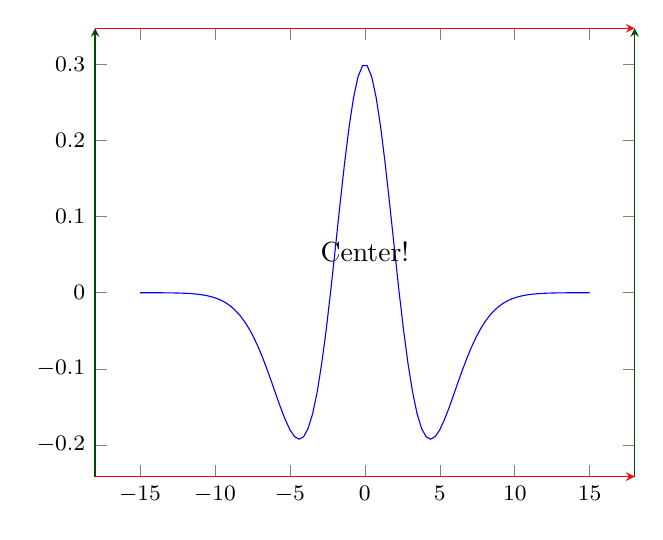
\begin{tikzpicture}
\begin{axis}[
	separate axis lines,
	every outer x axis line/.append style=
		{-stealth,red},
	every outer y axis line/.append style=
		{-stealth,green!30!black},
]
\addplot[blue,
		samples=100,
		domain=-15:15] 
	{1.3*exp(0-x^2/10) - exp(0-x^2/20)};
  % Unfortunately, there is a bug in PGF 2.00
  % something like exp(-10^2)
  % must be written as exp(0-10^2) :-(
\end{axis}
\end{tikzpicture}
\end{codeexample}

	The case |separate axis lines=false| issues just \emph{one} path for all axis lines. It draws a kind of rectangle, where some parts of the rectangle may be skipped over if they are not wanted. The advantage is that edges are closed properly. The disadvantage is that at most one arrow head is added to the path (and yes, only one drawing color is possible).
\begin{codeexample}[]
\begin{tikzpicture}
\begin{axis}[
	separate axis lines=false,
	every outer x axis line/.append style=
		{-stealth,red},
	every outer y axis line/.append style=
		{-stealth,green!30!black},
]
\addplot[blue,id=DoG,
		samples=100,
		domain=-15:15] 
  gnuplot{1.3*exp(-x**2/10) - exp(-x**2/20)};
\end{axis}
\end{tikzpicture}
\end{codeexample}
\end{pgfplotskey}


\label{pgfplots:page:axislines}
\begin{pgfplotskey}{axis line style=\marg{key-value-list}}
	A command which appends \marg{key-value-list} to \emph{all} axis line appearance styles.
\end{pgfplotskey}

\begin{pgfplotskey}{inner axis line style=\marg{key-value-list}}
	A command which appends \marg{key-value-list} to both, |every inner x axis line| and the $y$ variant.
\end{pgfplotskey}
\begin{pgfplotskey}{outer axis line style=\marg{key-value-list}}
	A command which appends \marg{key-value-list} to both, |every outer x axis line| and the $y$ variant.
\end{pgfplotskey}
\begin{pgfplotsxykey}{\x\ axis line style=\marg{key-value-list}}
	A command which appends \marg{key-value-list} to all axis lines styles for either $x$ or $y$ axis.
\end{pgfplotsxykey}

\begin{pgfplotsxykey}{every boxed \x\ axis}
	A style which will be installed as soon as |axis x line=box| (|y|) is set.

	The default is simply empty.
\end{pgfplotsxykey}
\begin{pgfplotsxykey}{every non boxed \x\ axis}
	A style which will be installed as soon as |axis x line| (|y|) will be set to something different than |box|. 
	
	The default is 
\begin{codeexample}[code only]
\pgfplotsset{
	every non boxed x axis/.style={
		xtick align=center,
		enlarge x limits=false,
		x axis line style={-stealth}}}
\end{codeexample}
	\noindent with similar values for the |y|-variant. Feel free to redefine this style to your needs / taste.
\end{pgfplotsxykey}

\subsubsection[Two Ordinates]{Two Ordinates ($y$ axis)}
{%
\pgfplotsset{every axis/.append style={width=4.5cm}}%
In some applications, more than one $y$ axis is used if the $x$ range is the same. This section demonstrates how to create them.

\begin{codeexample}[]
\begin{tikzpicture}
  \begin{axis}[
    scale only axis,
    xmin=-5,xmax=5,
    axis y line=left,
    xlabel=$x$,
    ylabel=First ordinate]
  \addplot {x^2};
  \end{axis}
  
  \begin{axis}[
    scale only axis,
    xmin=-5,xmax=5,
    axis y line=right,
    axis x line=none,
    ylabel=Second ordinate]
  \addplot[red] {3*x};
  \end{axis}
\end{tikzpicture}
\end{codeexample}
\noindent The basic idea is to draw two axis ``on top'' of each other -- one, which contains the $x$ axis and the left $y$ axis, and one which has \emph{only} the right $y$ axis. Since \PGFPlots\ does not really know what it's doing here, user attention in the following possibly non-obvious aspects is required:
\begin{enumerate}
	\item Scaling. You should set |scale only axis| because this forces equal dimensions for both axis, without respecting any labels.
	\item Same $x$ limits. You should set those limits explicitly.
\end{enumerate}
You may want to consider different legend styles.
It is also possible to use only the axis, without any plots:
% \usepackage{textcomp}
\begin{codeexample}[]
% \usepackage{textcomp}
\begin{tikzpicture}
  \begin{axis}[
    scale only axis,
    xmin=-5,xmax=5,
    axis y line=left,
    xlabel=$x$,
    ylabel=Absolute]
  \addplot {x^2};
  \end{axis}
  
  \begin{axis}[
    scale only axis,
    xmin=-5,xmax=5,
    ymin=0,ymax=1000,
    yticklabel=
{$\pgfmathprintnumber{\tick}$\textperthousand},
    axis y line=right,
    axis x line=none,
    y label style={yshift=-10pt},
    ylabel=per thousand]
  \end{axis}
\end{tikzpicture}
\end{codeexample}
}

\subsubsection{Axis Discontinuities}
In case the range of either of the axis do not include the zero value, it is possible to visualize this with a discontinuity decoration on the corresponding axis line.

\begin{pgfplotsxykey}{axis \x\ discontinuity=\mchoice{crunch,parallel,none} (initially none)}
Insert a discontinuity decoration on the $x$ (or $y$, respectively) axis. 
This is to visualize that the $y$ axis does cross the $x$ axis at its $0$ value, because the minimum $x$ axis value is positive or the maximum value is negative.

The description applies |axis y discontinuity| as well, with interchanged meanings of $x$~and~$y$.

\begin{codeexample}[]
\begin{tikzpicture}
\begin{axis}[
	axis x line=bottom,
	axis x discontinuity=parallel,
	axis y line=left,
	xmin=360, xmax=600,
	ymin=0, ymax=7,
 	enlargelimits=false
]
	\addplot coordinates {
		(420,2)
		(500,6)
		(590,4)
	};
\end{axis}
\end{tikzpicture}
\end{codeexample}

\begin{codeexample}[]
\begin{tikzpicture}
\begin{axis}[
	axis x line=bottom,
	axis y line=center,
	tick align=outside,
	axis y discontinuity=crunch,
	ymin=95, enlargelimits=false
]
	\addplot[blue,mark=none,
		 domain=-4:4,samples=20] 
		{x*x+x+104};
\end{axis}
\end{tikzpicture}
\end{codeexample}
\end{pgfplotsxykey}

A problem might occur with the placement of the ticks on the axis.
This can be solved by specifying the minimum or maximum axis value for which a tick will be placed.

\begin{pgfplotsxykeylist}{\x tickmin=\marg{coord} (default axis limits), \x tickmax=\marg{coord} (default axis limits)}
\label{key:xytickminmax}
The options |xtickmin|, |xtickmax| and |ytickmin|, |ytickmax| allow to define the axis tick limits, i.e.\ the axis values before respectively after no ticks will be placed.
Everything outside of the axis tick limits will be not drawn.
Their default values are equal to the axis limits.

\begin{codeexample}[]
\begin{tikzpicture}
\begin{axis}[
	axis x line=bottom,
	axis y line=center,
	tick align=outside,
	axis y discontinuity=crunch,
	xtickmax=3,
	ytickmin=110,
	ymin=95, enlargelimits=false
]
	\addplot[blue,mark=none,
		 domain=-4:4,samples=20] 
		{x*x+x+104};
\end{axis}
\end{tikzpicture}
\end{codeexample}
\end{pgfplotsxykeylist}

\begin{pgfplotsxykey}{hide \x\ axis=\mchoice{true,false} (initially false)}
Allows to hide either the $x$ or the $y$ axis. No outer rectangle, no tick marks and no labels will be drawn. Only titles and legends will be processed as usual.

Axis scaling and clipping will be done as if you did not use |hide x axis|.
\begin{codeexample}[]
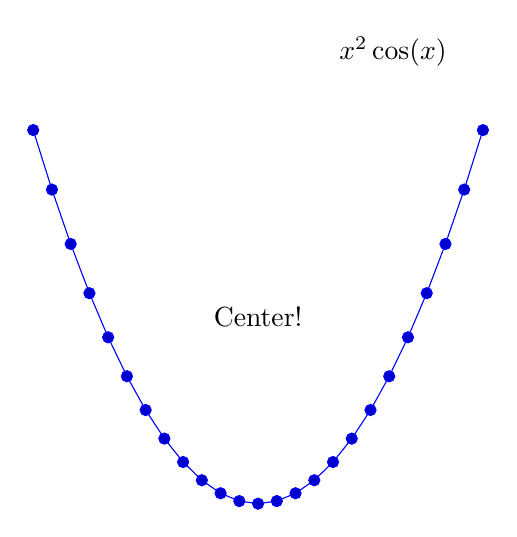
\begin{tikzpicture}
	\begin{axis}[
		hide x axis,
		hide y axis,
		title={$x^2\cos(x)$}]
	\addplot {cos(x)*x^2};
	\end{axis}
\end{tikzpicture}
\end{codeexample}

\begin{codeexample}[]
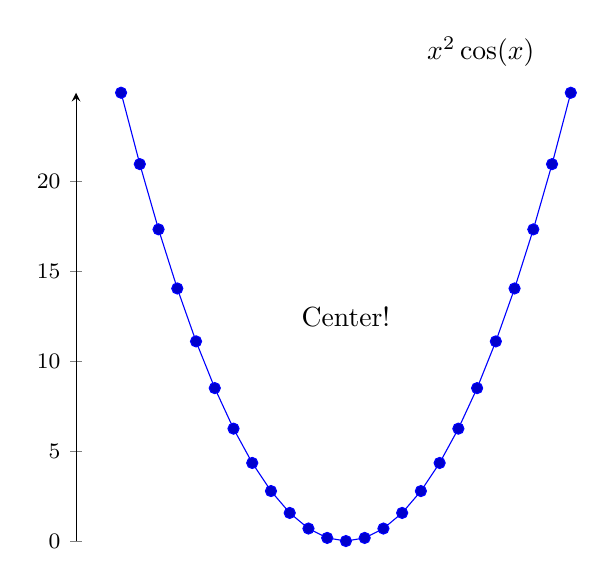
\begin{tikzpicture}
	\begin{axis}[
		hide x axis,
		axis y line=left,
		title={$x^2\cos(x)$}]
	\addplot {cos(x)*x^2};
	\end{axis}
\end{tikzpicture}
\end{codeexample}
\end{pgfplotsxykey}

\begin{stylekey}{/pgfplots/hide axis=\mchoice{true,false} (default true)}
	A style which sets both, |hide x axis| and |hide y axis|.
\end{stylekey}

\subsubsection{Color Bars}
\label{pgfplots:colorbar}
\PGFPlots\ supports mesh, surface and scatter plots which can use color maps. While color maps can be chosen as described in section~\ref{pgfplots:colormap}, they can be visualized using color bars.

\begin{pgfplotskey}{colorbar=\mchoice{true,false} (initially false)}
	Activates or deactivates color bars.

\begin{codeexample}[]
\begin{tikzpicture}
	\begin{axis}[colorbar]
		\addplot[mesh,ultra thick] {x};
	\end{axis}
\end{tikzpicture}
\end{codeexample}

\begin{codeexample}[]
\begin{tikzpicture}
	\begin{axis}[colorbar,colormap/greenyellow]
		\addplot[mesh,ultra thick] {x};
	\end{axis}
\end{tikzpicture}
\end{codeexample}

\begin{codeexample}[]
\begin{tikzpicture}
	\begin{axis}[colorbar horizontal]
		\addplot[mesh,ultra thick] {x};
	\end{axis}
\end{tikzpicture}
\end{codeexample}
	
	A color bar is only useful for plots which actually use color data -- that is, the special data which is called ``point meta'' in \PGFPlots\ (see section~\ref{pgfplots:point:meta}). Activating color bars for a plot without color map results in an empty color bar.

	Color bars are just normal axes which are placed right besides their parent axes. The only difference is that they inherit several styles such as line width and fonts and they contain a bar shaded with the color map of the current axis.
	
	Color bars are drawn internally with
\begin{codeexample}[code only]
\axis[every colorbar,colorbar shift,colorbar=false]
	\addplot graphics {};
\endaxis
\end{codeexample}
	\noindent where the placement, alignment, appearance and other options are done by the two styles |every colorbar| and |colorbar shift|. These styles and the possible placement and alignment options are described below.

	\paragraph{Remarks for special cases:}
	\begin{itemize}
		\item Since there is always only one color bar per plot, this color bar uses the axis wide configurations of color map and color data.
		\item If someone needs more than one color bar, the draw command above needs to be updated. See the key 
		|colorbar/draw/.code| for this special case.
	\end{itemize}
\end{pgfplotskey}

\begin{stylekey}{/pgfplots/colorbar right}
	A style which defines |every colorbar| and |colorbar shift| such that color bars are placed right of their parent axis.

	This is the initial configuration.
\begin{codeexample}[]
\begin{tikzpicture}
	\begin{axis}[colorbar right]
	\addplot[mesh,thick,samples=150,domain=0.1:3] 
		{1/x};
	\end{axis}
\end{tikzpicture}
\end{codeexample}
	
	The style |colorbar right| is defined to be
\begin{codeexample}[code only]
\pgfplotsset{
	colorbar right/.style={%
		/pgfplots/colorbar=true,
		/pgfplots/colorbar shift/.style={xshift=0.3cm},
		/pgfplots/every colorbar/.style={%
			title=,
			xlabel=,
			ylabel=,
			zlabel=,
			legend entries=,
			axis on top,
			at={(parent axis.right of north east)},
			anchor=north west,
			xmin=0,
			xmax=1,
			ymin=\pgfkeysvalueof{/pgfplots/point meta min},
			ymax=\pgfkeysvalueof{/pgfplots/point meta max},
			plot graphics/xmin=0,%
			plot graphics/xmax=1,
			plot graphics/ymin=\pgfkeysvalueof{/pgfplots/point meta min},
			plot graphics/ymax=\pgfkeysvalueof{/pgfplots/point meta max},
			enlargelimits=false,
			scale only axis,
			height=\pgfkeysvalueof{/pgfplots/parent axis height},%
			x=\pgfkeysvalueof{/pgfplots/colorbar/width},
			yticklabel pos=right,
			xtick=\empty,
			colorbar vertical/lowlevel,
		}%
	},%
	/pgfplots/colorbar vertical/lowlevel/.style={%
		plot graphics/lowlevel draw/.code 2 args={%
			\pgfplotscolormaptoshadingspec{\pgfkeysvalueof{/pgfplots/colormap name}}{##2}\pgfplots@loc@TMPa
			\def\pgfplots@loc@TMPb{%
				\pgfdeclareverticalshading{tempshading}{\pgfkeysvalueof{/pgfplots/colorbar/width}}}%
			\expandafter\pgfplots@loc@TMPb\expandafter{\pgfplots@loc@TMPa}%
			\pgfuseshading{tempshading}%
		},%
	},
}
\end{codeexample}
\end{stylekey}

\begin{stylekey}{/pgfplots/colorbar left}
	A style which defines |every colorbar| and |colorbar shift| such that color bars are placed left of their parent axis.
\begin{codeexample}[]
\begin{tikzpicture}
	\begin{axis}[colorbar left]
	\addplot[mesh,thick,samples=150] 
		{x*sin(deg(4*x))};
	\end{axis}
\end{tikzpicture}
\end{codeexample}
	
	The style |colorbar left| is defined to be
\begin{codeexample}[code only]
\pgfplotsset{
	colorbar left/.style={%
		/pgfplots/colorbar right,
		/pgfplots/colorbar shift/.style={xshift=-0.3cm},
		/pgfplots/every colorbar/.append style={%
			at={(parent axis.left of north west)},
			anchor=north east,
			yticklabel pos=left,
		}%
	}%
}
\end{codeexample}
\end{stylekey}

\begin{stylekey}{/pgfplots/colorbar horizontal}
	A style which defines |every colorbar| and |colorbar shift| such that color bars are placed below their parent axis, with a horizontal bar.
\begin{codeexample}[]
\begin{tikzpicture}
	\begin{axis}[colorbar horizontal]
	\addplot[only marks,scatter,
		scatter src={mod(\coordindex,15)},samples=150] 
		{rand};
	\end{axis}
\end{tikzpicture}
\end{codeexample}

	This style is defined to be
\begin{codeexample}[code only]
\pgfplotsset{
	colorbar horizontal/.style={%
		/pgfplots/colorbar=true,
		/pgfplots/colorbar shift/.style={yshift=-0.3cm},
		/pgfplots/every colorbar/.style={%
			title=,
			xlabel=,
			ylabel=,
			zlabel=,
			legend entries=,
			axis on top,
			at={(parent axis.below south west)},
			anchor=north west,
			ymin=0,
			ymax=1,
			xmin=\pgfkeysvalueof{/pgfplots/point meta min},
			xmax=\pgfkeysvalueof{/pgfplots/point meta max},
			plot graphics/ymin=0,%
			plot graphics/ymax=1,
			plot graphics/xmin=\pgfkeysvalueof{/pgfplots/point meta min},
			plot graphics/xmax=\pgfkeysvalueof{/pgfplots/point meta max},
			enlargelimits=false,
			scale only axis,
			width=\pgfkeysvalueof{/pgfplots/parent axis width},%
			y=\pgfkeysvalueof{/pgfplots/colorbar/width},
			xticklabel pos=left,
			ytick=\empty,
			colorbar horizontal/lowlevel,
		}%
	},%
	/pgfplots/colorbar horizontal/lowlevel/.style={%
		plot graphics/lowlevel draw/.code 2 args={%
			\pgfplotscolormaptoshadingspec{\pgfkeysvalueof{/pgfplots/colormap name}}{##1}\pgfplots@loc@TMPa
			\def\pgfplots@loc@TMPb{%
				\pgfdeclarehorizontalshading{tempshading}{\pgfkeysvalueof{/pgfplots/colorbar/width}}}%
			\expandafter\pgfplots@loc@TMPb\expandafter{\pgfplots@loc@TMPa}%
			\pgfuseshading{tempshading}%
		},%
	},%
}
\end{codeexample}
\end{stylekey}

\begin{stylekey}{/pgfplots/every colorbar}
	This style governs the placement, alignment and appearance of color bars. Any desired detail changes for color bars can be put into this style. Additionally, there is a style |colorbar shift| which is set after |every colorbar|. The latter style is intented to contain only shift transformations like |xshift| or |yshift| (making it easier to overwrite or deactivate them).

	While a color bar is drawn, the predefined node |parent axis| can be used to align at the parent axis.
\begin{predefinednode}{parent axis}
	A node for the parent axis of a color bar. It is only valid for color bars.
\end{predefinednode}

	Thus, 
\begin{codeexample}[code only]
\pgfplotsset{
	colorbar style={
		at={(parent axis.right of north east)},
		anchor=north west,
	},
	colorbar shift/.style={xshift=0.3cm}
}
\end{codeexample}
	\noindent places the colorbar in a way that its top-left (north west) corner is aligned right of the top right corner (|right of north east|) of its parent axis. Combining this with the |colorbar shift| is actually the same as the initial setting.

	Since color bars depend on some of its parent's properties, these properties are available as values of the following keys:
\begin{pgfplotskeylist}{point meta min,point meta max}
	The values of these keys contain the lower and upper bound of the color map, i.e.\ the lower and upper limit for the color bar. 
	
	The value is |\pgfkeysvalueof{/pgfplots/point meta min}| inside of |every colorbar|.
\end{pgfplotskeylist}
\begin{pgfplotskeylist}{parent axis width,parent axis height}
	The values of these keys contain the size of the parent axis. They can be used as |width| and/or |height| arguments for |every colorbar| with |\pgfkeysvalueof{/pgfplots/parent axis width}|.

	These values are only valid inside of color bars.
\end{pgfplotskeylist}

	Besides these values, each color bar inherits a list of styles of its parent axis, namely

	\begin{itemize}
		\item |every tick|,
		\item |every minor tick|,
		\item |every major tick|,
		\item |every axis grid|,
		\item |every minor grid|,
		\item |every major grid|,
		\item |every tick label|.
	\end{itemize}
	This can be used to inherit line width and/or fonts.

	Please take a look at the predefined styles for |every colorbar| for examples.

	\paragraph{Remark:} A color bar is just a normal axis. That means |every colorbar| can contain specifications where to place tick labels, extra ticks, scalings and most other features of a normal axis as well (except nested color bars).
\end{stylekey}

\begin{pgfplotskey}{colorbar style=\marg{key-value list}}
	A shortcut for |every colorbar/.append style=|\marg{key-value list}. It appends options to the colorbar style.
\end{pgfplotskey}

\begin{pgfplotskey}{colorbar/width=\marg{dimension} (initially 0.5cm)}
	Sets the width of a color bar.
\pgfplotsexpensiveexample
\begin{codeexample}[]
\begin{tikzpicture}
	\begin{axis}[
		view/az=45,
		colorbar,
		colorbar/width=2cm,
		colormap/blackwhite]

	\addplot3[surf,domain=0:1,y domain=-3:3] {x*(1-x)*tanh(y)};
	\end{axis}
\end{tikzpicture}
\end{codeexample}

	For vertical color bars, this sets the height.
\end{pgfplotskey}


\begin{stylekey}{/pgfplots/colorbar shift}
	This style is installed after |every colorbar|. It is intented to contain only shift transformations like |xshift| and/or |yshift|. The reason to provide two separate styles is to allow easier deactivation of shift transformations.

\begin{codeexample}[code only]
\pgfplotsset{
	colorbar shift/.style={xshift=1cm}
}
\end{codeexample}
\end{stylekey}

\begin{predefinednode}{current colorbar axis}
	A predefined node for the color bar of an axis. After |\end{axis}|, this node can be used to align further graphical elements at the color bar. Note that |current axis| refers to the axis as such while |current colorbar axis| refers to the color bar (which is an axis itsself).
\end{predefinednode}

\begin{pgfplotscodekey}{colorbar/draw}
	This code key belongs to the low level interface of colorbars. It is invoked whenever a color bar needs to be drawn. Usually, it won't be necessary to use or modify this key explicitly.
	
	In the context when this key is invoked, the styles inherited from the parent axis are already set and the required variables (see the documentation of |every colorbar|) are initialised.

	This code key can be replaced if one needs more than one color bar (or other wrinkles).

	The initial configuration is
\begin{codeexample}[code only]
\pgfplotsset{colorbar/draw/.code={%
	\axis[every colorbar,colorbar shift,colorbar=false]
	\addplot graphics {};
	\endaxis
	}
}
\end{codeexample}

	Please note that a color bar axis is nothing special as such -- it is just a normal axis with one |plot graphics| command and it is invoked with a special set of options. The only special thing is that a set of styles and some variables are inherited from its parent axis.
\end{pgfplotscodekey}

\subsubsection{Scaling Descriptions: Predefined Styles}
\label{sec:scaling:styles}
It is reasonable to change font sizes, marker sizes etc. together with the overall plot size: Large plots should also have larger fonts and small plots should have small fonts and a smaller distance between ticks.

\begin{keylist}{
	/tikz/font=\mchoice{\textbackslash normalfont,\textbackslash small,\textbackslash tiny,$\dotsc$},
	/pgfplots/max space between ticks=\marg{integer},
	/tikz/mark size=\marg{integer}}
	These keys should be adjusted to the figure's dimensions. Use 
\begin{codeexample}[code only]
\pgfplotsset{tick label style={font=\footnotesize},
	label style={font=\small},
	legend style={font=\small}
}
\end{codeexample}
	to provide different fonts for different descriptions.

	The |max space between ticks| is described on page~\pageref{maxspacebetweenticks} and configures the approximate distance between successive tick labels (in |pt|). Please omit the |pt| suffix here.
\end{keylist}

There are a couple of predefined scaling styles which set some of these options:

\begin{stylekey}{/pgfplots/normalsize}
	Re-initialises the standard scaling options of \PGFPlots.

\begin{codeexample}[]
\begin{tikzpicture}
	\begin{axis}[normalsize,
		title=A ``normalsize'' figure,
		xlabel=The $x$ axis,
		ylabel=The $y$ axis,
		minor tick num=1,
		legend entries={Leg}]
		\addplot {max(4*x,7*x)};
	\end{axis}
\end{tikzpicture}
\end{codeexample}

	The initial setting is
\begin{codeexample}[code only]
\pgfplotsset{
	normalsize/.style={
		/pgfplots/width=240pt,
		/pgfplots/height=207pt,
		/pgfplots/max space between ticks=35
	}
}
\end{codeexample}
\end{stylekey}

\begin{stylekey}{/pgfplots/small}
	Redefines several keys such that the axis is ``smaller''.

\begin{codeexample}[]
\begin{tikzpicture}
	\begin{axis}[small,
		title=A ``small'' figure,
		xlabel=The $x$ axis,
		ylabel=The $y$ axis,
		minor tick num=1,
		legend entries={Leg}]
		\addplot {x^2};
	\end{axis}
\end{tikzpicture}
\end{codeexample}
	The initial setting is
\begin{codeexample}[code only]
\pgfplotsset{
	small/.style={
		/pgfplots/width=6.5cm,
		/pgfplots/height=,
		/pgfplots/max space between ticks=25
	}
}
\end{codeexample}
Feel free to redefine the scaling -- the option may still be useful to get more ticks without typing too much. You could, for example, set |small,width=6cm|.
\end{stylekey}

\begin{stylekey}{/pgfplots/footnotesize}
	Redefines several keys such that the axis is even smaller. The tick labels will have |\footnotesize|.

\begin{codeexample}[]
\begin{tikzpicture}
	\begin{axis}[footnotesize,
		title=A ``footnotesize'' figure,
		xlabel=The $x$ axis,
		ylabel=The $y$ axis,
		minor tick num=1,
		legend entries={Leg}]
		\addplot+[const plot]
			coordinates {
			(0,0) (1,1) (3,3) (5,10)
		};
	\end{axis}
\end{tikzpicture}
\end{codeexample}
	The initial setting is
\begin{codeexample}[code only]
\pgfplotsset{
	footnotesize/.style={
		/pgfplots/width=5cm,
		/pgfplots/height=,
		legend style={font=\footnotesize},
		tick label style={font=\footnotesize},
		label style={font=\small},
		/pgfplots/max space between ticks=20,
		every mark/.append style={mark size=8},
		major tick length=0.1cm,
		minor tick length=0.066cm,
	},
}
\end{codeexample}
As for |small|, it can be convenient to set |footnotesize| and set |width| afterwards.

See also the |compat=newest| method which causes the positions of |xlabel|, |ylabel| and |zlabel| to be right near the tick labels.
\end{stylekey}
